%%%%%%%%%%%%%%%%%%%%%%%%%%%%%%% beamer %%%%%%%%%%%%%%%%%%%%%%%%%%%%%%%%%%%%%%%%%%%%%%%%%
% To run - pdflatex filename.tex
%      acroread filename.pdf
%%%%%%%%%%%%%%%%%%%%%%%%%%%%%%%%%%%%%%%%%%%%%%%%%%%%%%%%%%%%%%%%%%%%%%%%%%%%%%%%%%%%%%%%

\documentclass[compress,oilve]{beamer}
\mode<presentation>

\usetheme[]{CambridgeUS}
% other themes: AnnArbor, Antibes, Bergen, Berkeley, Berlin, Boadilla, boxes, CambridgeUS, Copenhagen, Darmstadt, default, Dresden, Frankfurt, Goettingen,
% Hannover, Ilmenau, JuanLesPins, Luebeck, Madrid, Maloe, Marburg, Montpellier, PaloAlto, Pittsburg, Rochester, Singapore, Szeged, classic

\usecolortheme{beaver}
% color themes: albatross, beaver, beetle, crane, default, dolphin,  fly, lily, orchid, rose, seagull, seahorse, sidebartab, whale, wolverine

\usefonttheme{professionalfonts}
% font themes: default, professionalfonts, serif, structurebold, structureitalicserif, structuresmallcapsserif


\hypersetup{pdfpagemode=FullScreen} % makes your presentation go automatically to full screen

% define your own colors:
\definecolor{Red}{rgb}{1,0,0}
\definecolor{Blue}{rgb}{0,0,1}
\definecolor{Green}{rgb}{0,1,0}
\definecolor{magenta}{rgb}{1,0,.6}
\definecolor{lightblue}{rgb}{0,.5,1}
\definecolor{lightpurple}{rgb}{0.8, 0.6, 0.9}
\definecolor{gold}{rgb}{.6,.5,0}
\definecolor{orange}{rgb}{1,0.4,0}
\definecolor{hotpink}{rgb}{1,0,0.5}
\definecolor{newcolor2}{rgb}{.5,.3,.5}
\definecolor{newcolor}{rgb}{0,.3,1}
\definecolor{newcolor3}{rgb}{1,0,.35}
\definecolor{darkgreen1}{rgb}{0, .35, 0}
\definecolor{darkgreen}{rgb}{0, .6, 0}
\definecolor{darkred}{rgb}{.75,0,0}
\definecolor{skyblue}{HTML}{75bbfd}

\definecolor{olive}{cmyk}{0.64,0,0.95,0.4}
\definecolor{purpleish}{cmyk}{0.75,0.75,0,0}

% can also choose different themes for the "inside" and "outside"

% \usepackage{beamerinnertheme_______}
% inner themes include circles, default, inmargin, rectangles, rounded

% \usepackage{beamerouterthemesmoothbars}
% outer themes include default, infolines, miniframes, shadow, sidebar, smoothbars, smoothtree, split, tree


\useoutertheme[subsection=true, height=40pt]{smoothbars}

% to have the same footer on all slides
%\setbeamertemplate{footline}[text line]{STUFF HERE!}
\setbeamertemplate{footline}[text line]{} % makes the footer EMPTY
% include packages
%

%show the page numbers in footnote
%\addtobeamertemplate{navigation symbols}{}{%
%	\usebeamerfont{footline}%
%	\usebeamercolor[fg]{footline}%
%	\hspace{1em}%
%	\insertframenumber/\inserttotalframenumber
%}

\setbeamercolor{footline}{fg=purpleish}
\setbeamerfont{footline}{series=\bfseries}

%add color to curent subsection
\setbeamertemplate{section in head/foot}{\hfill\tikz\node[rectangle, fill=darkred, rounded corners=1pt,inner sep=1pt,] {\textcolor{white}{\insertsectionhead}};}
\setbeamertemplate{section in head/foot shaded}{\textcolor{darkred}{\hfill\insertsectionhead}}

% Remove bullet of subsections
\setbeamertemplate{headline}
{%
	\begin{beamercolorbox}{section in head/foot}
		\insertsectionnavigationhorizontal{\textwidth}{}{}
	\end{beamercolorbox}%
}


% modify headlline, specially headline size
\setbeamertemplate{headline}{%
	\leavevmode%
	\hbox{%
		\begin{beamercolorbox}[wd=\paperwidth,ht=3.5ex,dp=1.125ex]{palette quaternary}%
			\insertsectionnavigationhorizontal{\paperwidth}{}{\hskip0pt plus1filll}
		\end{beamercolorbox}%
	}
}

\setbeamertemplate{footline}{%
	\leavevmode%
	\hbox{\begin{beamercolorbox}[wd=.5\paperwidth,ht=2.5ex,dp=1.125ex,leftskip=.3cm plus1fill,rightskip=.3cm]{author in head/foot}%
			\usebeamerfont{author in head/foot}\insertshortauthor ~ \insertshortinstitute
		\end{beamercolorbox}%
		\begin{beamercolorbox}[wd=.5\paperwidth,ht=2.5ex,dp=1.125ex,leftskip=.3cm,rightskip=.3cm plus1fil]{title in head/foot}%
			\usebeamerfont{title in head/foot}\insertshorttitle\hfill\insertframenumber\,/\,\inserttotalframenumber
	\end{beamercolorbox}}%
	\vskip0pt%
}


%\setbeamertemplate{navigation symbols}{}

\title{Lecture 2: Introduction to ML and Classical Models}
\author{ML Instruction Team, Fall 2022}
\institute[]{CE Department \newline  Sharif University of Technology \newline \newline}
\date[\today]{}
%\titlegraphic{\includegraphics[scale=.35]{example-image}}



%Write \usepackage{etex} just after the \documentclass line (it should be the first loaded package).
\usepackage{etex}
\usepackage{subcaption}
\usepackage{multicol}
\usepackage{physics, amsmath}
\usepackage{epsfig}
\usepackage{graphicx}
\usepackage{amsfonts}
\usepackage{amssymb}
\usepackage[all,knot]{xy}
\xyoption{arc}
\usepackage{url}
\usepackage{multimedia}
\usepackage{hyperref}
\hypersetup{colorlinks,linkcolor=blue,citecolor=redorange,urlcolor=darkred}
\usepackage{multirow}
\usepackage[font={scriptsize}]{caption}
\usepackage{pgf}
\usepackage{fontspec}
\usepackage{subcaption}
\usepackage[export]{adjustbox}
\usepackage{caption}
%\setsansfont[Scale=MatchLowercase, BoldFont = * Bold, ItalicFont = * Italic]{Caladea}
\graphicspath{ {./Pictures/} }
%\usepackage{enumitem,xcolor}
%\newcommand{\labelitemi}{$\blacksquare$}
%\newcommand{\labelitemii}{$\diamond$}
%\newcommand{\labelitemiii}{$\square$}
%\newcommand{\labelitemiv}{$\ast$}
%\setbeamercolor*{item}{fg=red}
\usepackage{bm}

\usefonttheme{professionalfonts} 
\setbeamertemplate{itemize item}{\color{skyblue}$\blacksquare$}
\setbeamertemplate{itemize subitem}{\color{hotpink}$\blacktriangleright$}
\setbeamertemplate{itemize subsubitem}{\color{orange}$\bullet$}


\usepackage{anyfontsize}
\usepackage{t1enc}
\usepackage{tikz}
\usetikzlibrary{calc,trees,positioning,arrows,chains,shapes.geometric,decorations.pathreplacing,decorations.pathmorphing,shapes,matrix,shapes.symbols}



\newtheorem{proposition}[theorem]{Proposition}
\newtheorem{remark}[theorem]{Remark}
\newtheorem{assumption}[theorem]{Assumption}

\usepackage{fontspec,unicode-math}
\setmainfont[Scale=0.9]{Consolas}
\setmonofont[Scale=0.9]{Monaco}
\setsansfont[Scale=1]{Times New Roman}
\newcommand{\vect}[1]{\boldsymbol{#1}}


%\usepackage{smartdiagram}
%\usesmartdiagramlibrary{additions}
%%%%%%%%%%%%%%%%%%%%%%%%%%%%%%%%%%%%%%%%%%%%%%%%%%%%%%%%%%%%%%%%%%%%%%%%%%%%%%%%%%%%%%%%%%%%
%%%%%%%%%%%%%%%%%%%%%%%%%%%%%% Title Page Info %%%%%%%%%%%%%%%%%%%%%%%%%%%%%%%%%%%%%%%%%%%
%%%%%%%%%%%%%%%%%%%%%%%%%%%%%%%%%%%%%%%%%%%%%%%%%%%%%%%%%%%%%%%%%%%%%%%%%%%%%%%%%%%%%%%%%%


%%%%%%%%%%%%%%%%%%%%%%%%%%%%%%%%%%%%%%%%%%%%%%%%%%%%%%%%%%%%%%%%%%%%%%%%%%%%%%%%%%%%%%%%%%
%%%%%%%%%%%%%%%%%%%%%%%%%%%%%% Begin Your Document %%%%%%%%%%%%%%%%%%%%%%%%%%%%%%%%%%%%%%%
%%%%%%%%%%%%%%%%%%%%%%%%%%%%%%%%%%%%%%%%%%%%%%%%%%%%%%%%%%%%%%%%%%%%%%%%%%%%%%%%%%%%%%%%%%
\begin{document}
	
%%%%%%%%%%%%%%%%%%%%%%%%%%%%%%%%%%%%%%%%%%%%%%%%%%%%%%%%%%%%%%%%%%%%%%%%%%%%%%%%%%%%%%%%%%
	\fontsize{9}{9}
\begin{frame}[noframenumbering, plain]
	\titlepage
\end{frame}

%%%%%%%%%%%%%%%%%%%%%%%%%%%%%%%%%%%%%%%%%%%%%%%%%%%%%%%%%%%%%%%%%%%%%%%%%%%%%%%%%%%%%%%%%%
\section{Introduction}
%%%%%%%%%%%%%%%%%%%%%%%%%%%%%%%%%%%%%%%%%%%%%%%%%%%%%%%%%%%%%%%%%%%%%%%%######
\frame{\frametitle{Machine Learning: An Overview}
\begin{center}
What is Machine Learning?
\end{center}
}

%%%%%%%%%%%%%%%%%%%%%%%%%%%%%%%%%%%%%%%%%%%%%%%%%%%%%%%%
\begin{frame}{Machine Learning: An Overview}
\begin{itemize}
\item Let's review some inspirational quotions ... \\
\begin{itemize}
	\item \textit{“Machine learning is the hot new thing”} \\ \begin{center}
— John L. Hennessy, President of Stanford (2000–2016) \end{center}
	\item\textit{ “A breakthrough in machine learning would be worth ten Microsofts” }\\ \begin{center}
— Bill Gates, Microsoft Co-Founder  \end{center}
	\item \textit{“Computers are able to see, hear and learn.  Welcome to the future.” }\\ \begin{center}
— Dave Waters, Professor at University of Oxford \end{center}
	\item \textit{“If software ate the world, models will run it”}
\\ \begin{center}
— Steven A. Cohen and Matthew W. Granade, The Wallstreet Journal, 2018\end{center}
	\item ...
\end{itemize}	
\end{itemize}
\end{frame}

%\begin{frame}{Machine Learning: An Overview}
%\begin{itemize}
%\item[$\blacksquare$] Among these quotions that we have discussed, one seems more interesting and important:\\
%\begin{center} \textit{"Machine learning is the field of study that gives computers the ability to
%learn without being explicitly programmed”} \\ 
%— Arthur L. Samuel, AI pioneer, 1959 \end{center}
%\item[$\blacksquare$] But why does it seem important? why should computers be able to learn? waht do they really learn? \\
%\item[$\blacksquare$] We shall answer these questions through this lecture
%\end{itemize}
%\end{frame}


\begin{frame}{Machine Learning: An Overview}
\begin{itemize}
\item The main motivation which we develop (computer) programs is to automate various
kinds of (often tedious) processes.
\item So far, we have learned to program the computers. the analogy that we have been using is something similar to this:\\

\begin{center}
\begin{figure}
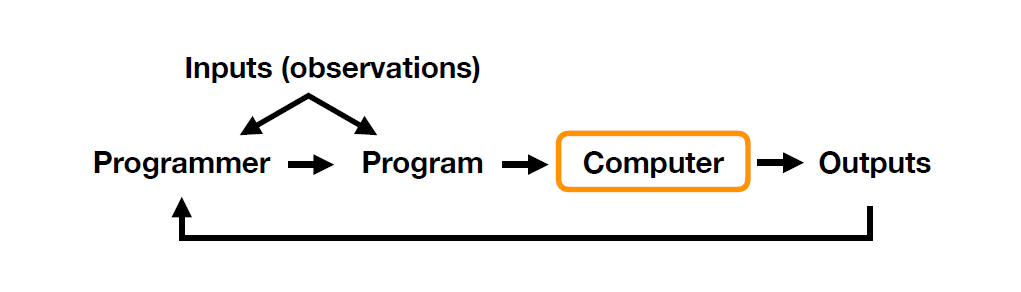
\includegraphics[scale=0.5]{1}
\caption{classical programming paradigm [1].}
\end{figure}
\end{center}
\end{itemize}
\end{frame}


\begin{frame}{Machine Learning: An Overview}
\begin{itemize}
\item The preceding traditional programming paradigm has several disadvantages:
	\begin{itemize}
	\item what if we don't know waht program should we write for the given data (inputs) ?
	\item what if the inputs change dynamically over the time? should we write another program? 
	\end{itemize}
\item In order to resolve such problems, we should replace the need of developing computer programs "manually"
\item In other words, we would like to automate the process of creating programs by informing the computer, the inputs and outputs that it needs:
\begin{center}
\begin{figure}
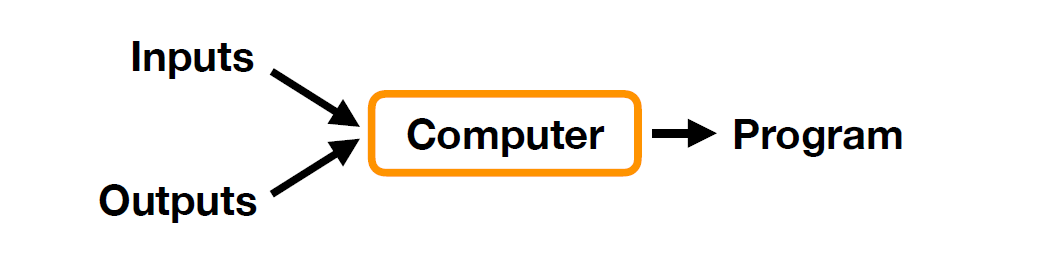
\includegraphics[scale=0.5]{2}
\center \caption{ML paradigm [1].}
\end{figure}
\end{center}
\end{itemize}
\end{frame}

\begin{frame}{Machine Learning: An Overview}
\begin{itemize}
\item The preceding model was the main function of Machine Learning paradigm, In fact ML systems use both inputs and outputs to discover the \textbf{Rules and Patterns} behind the data 
\item Now that we are fimiliar with ML paradigm, we would like to define it formally:
\begin{center}\textit{A computer program is said to learn from experience E with respect to some
class of tasks T and performance measure P, if its performance at tasks in T, as
measured by P, improves with experience E.}
\end{center}
\item Here, inputs and outputs would be the experience (\textit{E}), the main problem(s) that the computer wants to solve, is the class of tasks (\textit{T}) and finally the performance measure shows how computer succeeded in performing (\textit{P})
\end{itemize}
\end{frame}



%%%%%%%%%%%%%%%%%%%%%%%%%%%%%%%%%%%%%%%%%%%%%%%%%%%%%%%%%%%%%%%%%%%%%%%%%%%%%%%%%%%%%%%%%%%%%%%

%%%%%%%%%%%%%


\begin{frame}{Categories of Machine Learning}
\begin{itemize}
\item The three broad categories of ML are summerized in:
\begin{itemize}
\item \textbf{Supervised Learning}
\item \textbf{Unsupervised Learning}  
\item \textbf{Reinforcement Learning} 
\end{itemize}
\end{itemize}
\begin{figure}
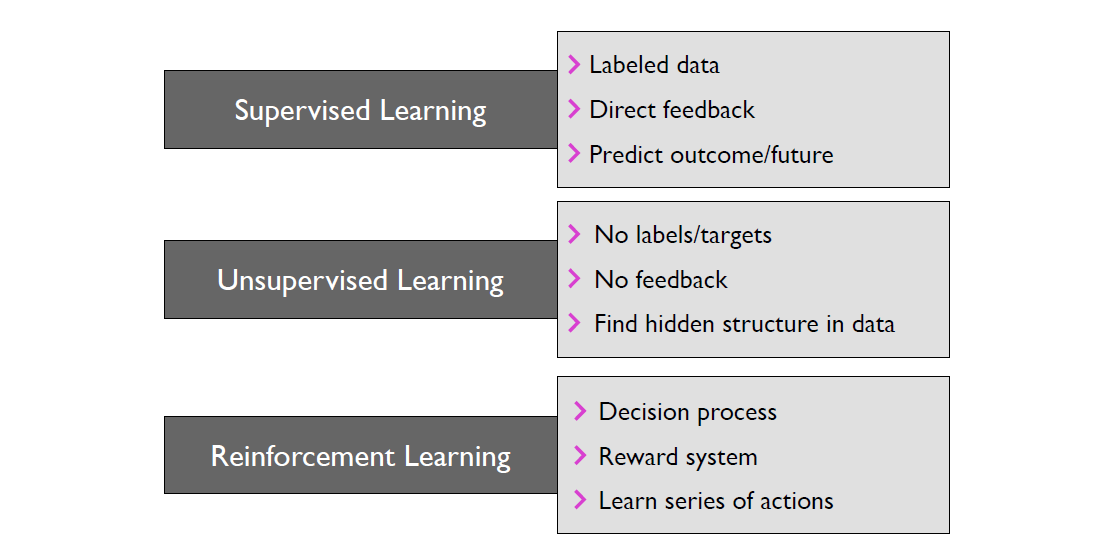
\includegraphics[scale=0.5, right]{3}
\caption{Categories of ML [2]}
\end{figure}
\end{frame}


\begin{frame}{Introduction to Supervised Learning}
\begin{itemize}
\item Supervised learning is the subcategory of machine learning that focuses on learning a \textbf{Classification} (Figure left), or \textbf{Regression} model (Figure right), that is, learning from labeled training data (i.e., inputs that also contain the desired outputs or targets; basically, "examples" of what we want to predict).
\end{itemize}
\begin{columns}
\begin{column}{0.5\textwidth}
\begin{figure}
 \centering
 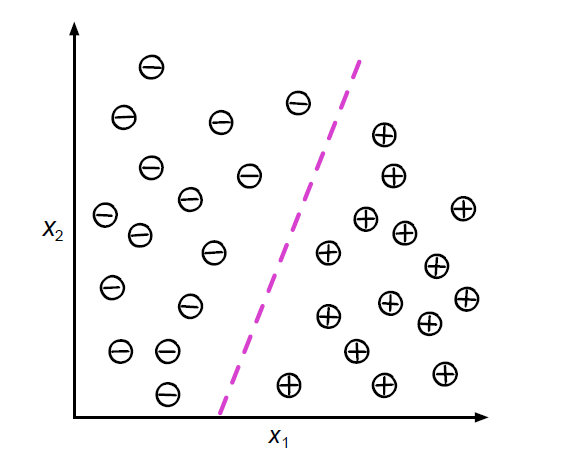
\includegraphics[scale=0.5]{10}  
 \caption{Illustration of classification problem [2].}
\end{figure}
\end{column}
\begin{column}{0.5\textwidth}
\begin{figure}
 \centering
 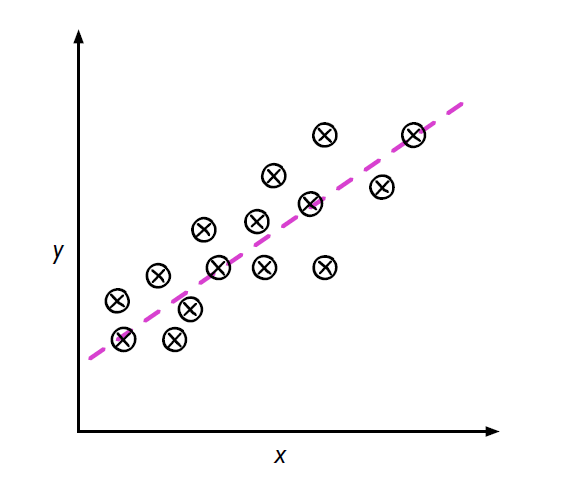
\includegraphics[scale=0.5]{11}  
 \caption{Illustration of a linear regression model [2].}
\end{figure}
\end{column}
\end{columns}
\end{frame}

\begin{frame}{Supervised Learning}
\begin{itemize}
\item Given a data set $ \mathcal{D} = \{ \langle \mathbf{x_{\mathnormal 1}} , y_{1} \rangle, \langle \mathbf{x_{\mathnormal 2}} , y_{2} \rangle, \dots, \langle \mathbf{x_{\mathnormal n}} , y_{n} \rangle\} $, there exists an unkown function called $ f $ which:
$$ y = f(\mathbf{x})$$
\item The supervised learning final goal is to \textbf{Approximate} this unkown function. we call our discovery function a \textit{hypothesis} and we define it:
$$  \begin{cases}
       h: \mathbb{R^{\mathnormal m}} \rightarrow \mathbb{R} \\
       h(\mathbf{x}) = y  
  \end{cases} $$
\end{itemize}
\end{frame}

\begin{frame}{Unsupervised Learning}
\begin{itemize}
\item In contrast to supervised learning, unsupervised learning is a branch of machine learning that is concerned with unlabeled data. Common tasks in unsupervised learning are \textbf{Clustering} analysis and \textbf{Dimensionality Reduction}.
\end{itemize}
\begin{columns}
\begin{column}{0.4\textwidth}
\begin{figure}
 \centering
 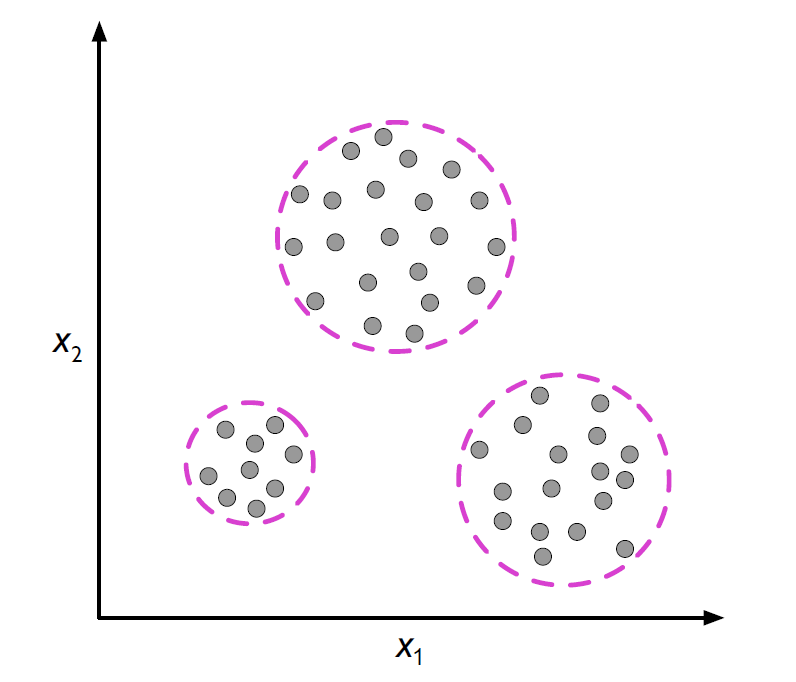
\includegraphics[scale=0.25]{14}  
 \caption{Illustration of Clustering [3].}
\end{figure}
\end{column}
\begin{column}{0.6\textwidth}
\begin{figure}
 \centering
 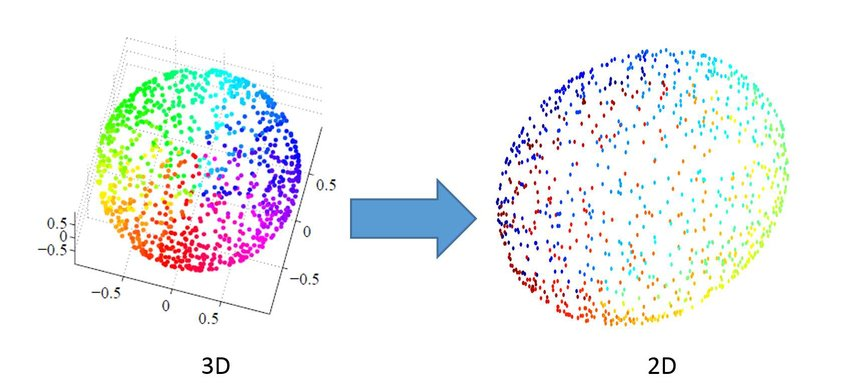
\includegraphics[scale=0.25]{16}  
 \caption{Illustration of Dimensionality Reduction [4].}
\end{figure}
\end{column}
\end{columns}
\end{frame}

\begin{frame}{Reinforcement Learning}
\begin{itemize}
\item Reinforcement is the process of learning from rewards while performing a series of actions.
\end{itemize}
\begin{figure}
 \centering
 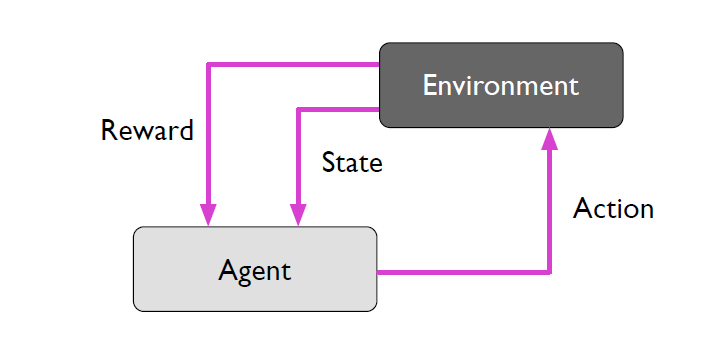
\includegraphics[scale=0.75]{15}  
 \caption{Illustration of Reinforcement Learning [2].}
\end{figure}
\end{frame}

\begin{frame}{Classes of Machine Learning Algorithms}
\begin{itemize}
\item Generalized linear models (e.g., logistic regression)
\item Support vector machines (e.g., linear SVM, RBF-kernel SVM)
\item Artificial neural networks (e.g., multi-layer perceptrons)
\item Tree- or rule-based models (e.g., decision trees)
\item Graphical models (e.g., Bayesian networks)
\item Ensembles (e.g., Random Forest)
\item Instance-based learners (e.g., K-nearest neighbors)
\end{itemize}
\end{frame}


\begin{frame}{Algorithm Categorization Schemes}
\begin{itemize}
\item Eager vs Lazy
\item Single-Task vs Multi-Task
\item Generative vs Discriminant
\item Instance-based vs Model-Based
\item Parametric vs Non-Parametric
\item Batch vs Online
\end{itemize}
\end{frame}

\begin{frame}{5 Steps To Solve A Machine Learning Problem}
\begin{itemize}
\item 1. Define the problem to be solved.
\item 2. Collect (labeled) data.
\item 3. Choose an algorithm class.
\item 4. Choose an optimization metric for learning the model.
\item 5. Choose a metric for evaluating the model.
\end{itemize}
\begin{figure}
 \centering
 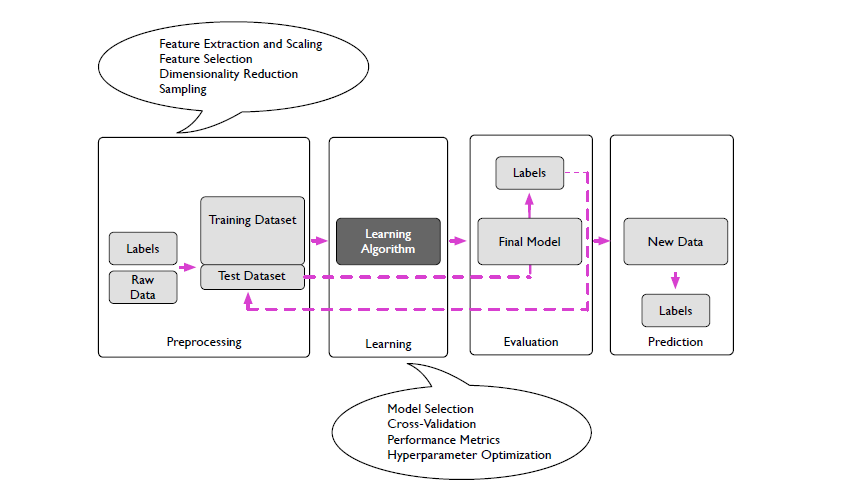
\includegraphics[scale=0.6]{13}  
 \caption{Learning Process [3].}
\end{figure}
\end{frame}

\begin{frame}{Objective Functions}
\begin{itemize}
\item Maximize the posterior probabilities (e.g., naive Bayes)
\item Maximize a fitness function (genetic programming)
\item Maximize the total reward/value function (reinforcement learning)
\item Maximize information gain/minimize child node impurities (CART decision tree classification)
\item Minimize a mean squared error cost (or loss) function (CART, decision tree regression, linear regression, adaptive linear neurons, ...)
\item Maximize log-likelihood or minimize cross-entropy loss (or cost) function
\item Minimize hinge loss (support vector machine)
\end{itemize}
\end{frame}


\begin{frame}{Optimization Methods}
\begin{itemize}
\begin{columns}
\begin{column}{0.5\textwidth}
\begin{itemize}
\item Combinatorial search, greedy search (e.g., decision trees over, not within nodes);
\item Unconstrained convex optimization (e.g., logistic regression);
\item Constrained convex optimization (e.g., SVM);
\item Nonconvex optimization, here: using backpropagation, chain rule, reverse autodi. (e.g., neural networks).
\item Constrained nonconvex optimization (semi-adversarial networks9, not covered in this course)
\end{itemize}
\end{column}
\end{columns}
\end{frame}

%%%%%%%%%%%%%%%%%%%%%%%%%%%%%%
\begin{frame}{Glossary}
\begin{itemize}
\item \textbf{Training example}: A row in the table representing the dataset. Synonymous to an observation, training record, training instance, training sample (in some contexts, sample refers to a collection of training examples).
\item \textbf{Training}: Model fitting, for parametric models similar to parameter estimation.
\item \textbf{Feature, $x$}: A column in the table representing the dataset. Synonymous to predictor, variable, input, attribute, independent variable, and covariate.
\item \textbf{Target}: Synonymous to outcome, output, response variable, dependent variable, (class) label, ground truth.
\item \textbf{Predicted output, $\hat{y}$}: Use this to distinguish from targets; here, means output from the model.
\item \textbf{Loss function}: Often used synonymously with cost function; sometimes also called error function. In some contexts the loss for a single data point, whereas the cost func- tion refers to the overall (average or summed) loss over the entire dataset. Sometimes also called empirical risk.

\end{itemize}
\end{frame}

\begin{frame}{Glossary}
\begin{itemize}
\item \textbf{Hypothesis:}: A hypothesis is a certain function that we believe (or hope) is similar to the true function, the target function that we want to model. In context of \textit{spam} classification, it would be a classification rule we came up with that allows us to separate spam from non-spam emails.

\item \textbf{Model}: In the machine learning field, the terms \textit{hypothesis} and \textit{model} are often used interchangeably. In other sciences, they can have different meanings: A hypothesis could be the "educated guess" by the scientist, and the model would be the manifestation of this guess to test this hypothesis.

\item \textbf{Learning algorithm}: Again, our goal is to find or approximate the target function, and the learning algorithm is a set of instructions that tries to model the target function using our training dataset. A learning algorithm comes with a hypothesis space, the set of possible hypothesis it explores to model the unknown target function by formulating the final hypothesis.

\end{itemize}
\end{frame}



\begin{frame}{Glossary}
\begin{itemize}

\item \textbf{Classifier}: A classifier is a special case of a hypothesis (nowadays, often learned by a machine learning algorithm). A classifier is a hypothesis or discrete-valued function that is used to assign (categorical) class labels to particular data points. In an email classification example, this classifier could be a hypothesis for labeling emails as spam or non-spam. Yet, a hypothesis must not necessarily be synonymous to the term \textit{classifier}. In a different application, our hypothesis could be a function for mapping study time and educational backgrounds of students to their future, continuous-valued, SAT scores - a continuous target variable, suited for regression analysis.
\item \textbf{Hyperparameters}: Hyperparameters are the \textit{tuning parameters} of a machine learning algorithm - for example, the regularization strength of an L2 penalty in the mean squared error cost function of linear regression, or a value for setting the maximum depth of a decision tree. In contrast, model parameters are the parameters that a learning algorithm fits to the training data - the parameters of the model itself. For example, the weight coeffcients (or slope) of a linear regression line and its bias (or y-axis intercept) term are \textit{model parameters}.
\end{itemize}
\end{frame}



\begin{frame}{References}
\begin{itemize}
\item Eager vs Lazy
\item Single-Task vs Multi-Task
\item Generative vs Discriminant
\item Instance-based vs Model-Based
\item Parametric vs Non-Parametric
\item Batch vs Online
\end{itemize}
\end{frame}

\frametitle{Final Notes}
\centering
\vspace{50 pt}
\textbf{Thank You!}
\vspace{50pt}

\textbf{Any Question?}
%%%%%%%%%%%%%%%%%%%%%%%%%%%%%%%%%%%%%%%%%%
\end{document}